%%%%%%%%%
% TO DO %
%%%%%%%%%
% Expand intro
% Redo graphs from graphing program, expand scope, involve 
% More detail
% Actually describe motivation again
% Rewrite into based off previous chapters


%Don't write too much
%Write what is needed in the text
%The more you write, the higher probability of making mistakes - keep to the point
%Describe results
%Explanation after desc
%Have to be phrases that make sense/say something
%Have a purpose

\chapter{Analysis of Approach Force Curves in Colloidal Systems}
\label{chap:approach_force_curves}

This chapter aims to serve a simple goal. To provide a clear route to extract the force at contact from raw data.  As the raw unprocessed data is severely voluminous the scope of this chapter is kept to one goal, provide the data and justification for the contact forces calculated for each concentration, site and parameter. The results of this analysis is then concluded in Chapter 7, which, is free of the need to justify every data point and thus focuses on the conclusions from this data. 

\section{MFP-1D contact force derivation}

For the data collected from the MFP-1D the analytical approach to this elucidation is given in Chapter 4. This section will overview the results for the following LiCl concentrations: 0.6mM, 1.6mM, 5mM, 10mM, 25mM, 50mM, 230mM, 550mM. For each concentration multiple sites are analysed, highlighting features of each curve in preparation for analysis. 

\subsection{A note one Rejected curves}

 During the process, several curves were rejected from the data set as part of the processing method. Due to the sheer volume of curves (10,000+ curves) involved in this analysis.  This was either due to machine failure to engage in the surface, or due to significant noise due to mechanical failure (over-correction in piezo movement by the AFM or vibrations in the building.) While the initial curves taken on the machine were too noisy, further repeats and refinements to the procedure eventually resulted in usable curves. In some of the data collected, the impact from residual vibrations was mitigated in later datasets by operating the AFM in the night. Other improvements were found by optimising the AFM parameters  - such as tip speed, data collection rate and target force. The optimal parameters found were 0.5Hz for tip speed, setting the data collection rate to maximum and a target force of 8-12nN. 

\begin{figure}
    \centering
    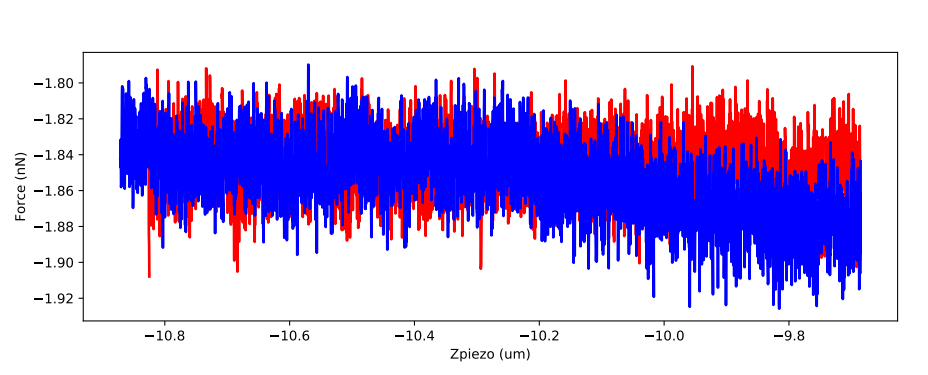
\includegraphics[width=0.65\linewidth]{chapter5/miss_error.png}
    \caption{A graph demonstrating a rejected curve. In this case the AFM failed to reach the surface for the recorded data, leading to a single up and down motion.}
    \label{fig:miss-error}
\end{figure}

The other reason for rejected curves was due to the shift of the snapshot window providing too little data in either the approach phase or the contact phase (covered in Chapter 4). 

\subsection{Contact force calculations}

In this results section, the contact force graphs displayed represent only a subset of the total analyzed graphs, selected to illustrate the most significant aspects of the analysis procedure. The ones chosen here represent the typical majority of the curves, with outliers not reflected in the dataset. Outliers may be demonstrated, and will be commented on if presented. The remainder of the curves, not shown here, played an instrumental role in guiding the parameter optimization process for the data processing script. This process involved the review and refinement of several hundred thousand curves in order to deal with the noise intrinsic to the system. Ensuring a good fit for these curves is paramount; otherwise, one risks obtaining erratic and misleading graphs that could compromise the integrity of the data interpretation. The selection process for the resulting curves involved the exclusion of certain outliers and repeat measurements, a necessary step taken to refine the data and enhance the clarity of the observed trends. Three types of graphs were chosen for their analysis of the fitting parameters and results: the histogram of contact forces provides a statistical view of the interaction forces at the point of contact, demonstrating the range of forces across the graph. The log-linear plot of the force as a function of the Z-piezo position (in nanometers), highlighting of the separation distance between the AFM tip and the sample surface during the interaction phase. At the top of the graph the transition to the contact phase can be seen. This point of transition is the contact force. The logarithmic scale for force highlights the sensitivity of the AFM in detecting forces at the nanoscale. Finally the overall approach force curve derived from binned data presents a view of the resulting averaged force curve behavior during the approach phase. Each graph was selected for its ability to support the chosen parameters and thus the resulting contact force.


%0.6mM
\insertapproachfigures{5}{0.6}{1}{Site one demonstrates one of the difficulties with collecting the data at the lower ranges of the molar concentrations. As the repulsive force is over a wider range there is a smaller window captured of the contact phase. This means that when trying to fit to the data, there is less data available to provide a solid fit.  As such, a slight bowing effect is seen in the binned average curve.}
\insertapproachfigures{5}{0.6}{2}{Site two demonstrates the lowest observed force for this concentration, highlighting a high degree of variability between sites.}
\insertapproachfigures{5}{0.6}{3}{Site three demonstrates an ideally fitted curve, however in the log-linear plot an irregularity is seen - the point in which the contact force area is raised up the graph. This is due to the large amount of noise seen during this interface phase, giving a large variation in the contact force histogram.}
% ... and so on for other sites and concentrations.

%1.6
\insertapproachfigures{5}{1.6}{1}{Site one represents an good example of a typical well-behaved curve, where the processing is able to extract out a clear signal from the noise, and thus a clearly distributed contact force.}
\insertapproachfigures{5}{1.6}{2}{Site 2 demonstrates an interesting feature - a region where there seems to be two contact phases. As DLVO doesn't explain any dual barrier features this is rather unexpected. One explanation may be that as the two surfaces approach one another some aspect (for example a small topographical protrusion or a small aggregate of ions) prevents full contact between the sphere and surface, which then slips or is overcome, allowing full contact later. It is important to note that this feature is present throughout the dataset, and survived the binning and averaging process, and thus is a consistent feature in this site.}

%5
\insertapproachfigures{5}{5}{1}{Site one demonstrates a similar, but weaker feature seen in 1.6mM site 2 observable in the log-lin plot. The overall binned fit demonstrates a suitable fit, so it remains to be a feature of this site. Equally, this site demonstrates the weakest repulsive force in the set.}
\insertapproachfigures{5}{5}{2}{Site two demonstrates the same feature, but slightly less prominent again.}
\insertapproachfigures{5}{5}{3}{Site three once again has the feature seen across all of the force curves at this concentration}

5mM presents an interesting and repeatable shelf seen in the force profiles across all different sites. There are a number of theories as to what this feature may be. For one If the AFM tip encounters a region of the sample with a topological feature that does not mesh well with the surface it could provide the observed barrier. This feature can then hold the tip back from fully sliding down until a threshhold force determined by the surface roughness is presented. Once this threshold force is overcome it then "slips" down futher into contact.

%10 2 sites
\insertapproachfigures{5}{10}{1}{Site 1 demonstrates a noisy top of the graph, which can sometimes happen when the AFM oversteers and provides too much force onto the sample.}
\insertapproachfigures{5}{10}{2}{}
\insertapproachfigures{5}{10}{3}{}

%25 3 sites
\insertapproachfigures{5}{25}{1}{Site 1 demonstrates a high degree of noise in the binned average curve and demonstrates towards what curves could be without the involved processing}
\insertapproachfigures{5}{25}{2}{Site 2 also demonstrates a shelf feature.}
\insertapproachfigures{5}{25}{3}{}

%50 2 sites
\insertapproachfigures{5}{50}{1}{}
\insertapproachfigures{5}{50}{2}{}

%230 2 sites
\insertapproachfigures{5}{230}{1}{}
\insertapproachfigures{5}{230}{2}{}

%550 3 sites
\insertsnowflakefigures{5}{550}{1}{500mM marks the situation where the charge screen starts to overcome the electrostatic repulsion, giving way to an attractive force instead. Interestingly the shelf effect is still observed despite the attractive nature of the two surfaces.}
\insertsnowflakefigures{5}{550}{2}{}
\insertsnowflakefigures{5}{550}{3}{}

\section{Overall force vs LiCl concentration graph}

The forces calculated at the point of contact were subsequently plotted on a graph. For the values, the average was taken, the standard deviation was calculated by:

\begin{equation}
Stdev_{avg} = \sqrt{\frac{{x_1}^2 + {x_2}^2 + {x_3}^2}{n_{num}}}  
\label{eq:Stdevavg}
\end{equation}

Where $x_{#}$ is the site's standard deviation and $n_{num}$ is the number of sites in the calculation (i.e. where there were 3 sites, this value was 3).

 In the case of a LiCl concentration of 550 mM, the attractive force was utilized in the plot due to the alteration in the nature of the force curve.

\begin{figure}
    \centering
    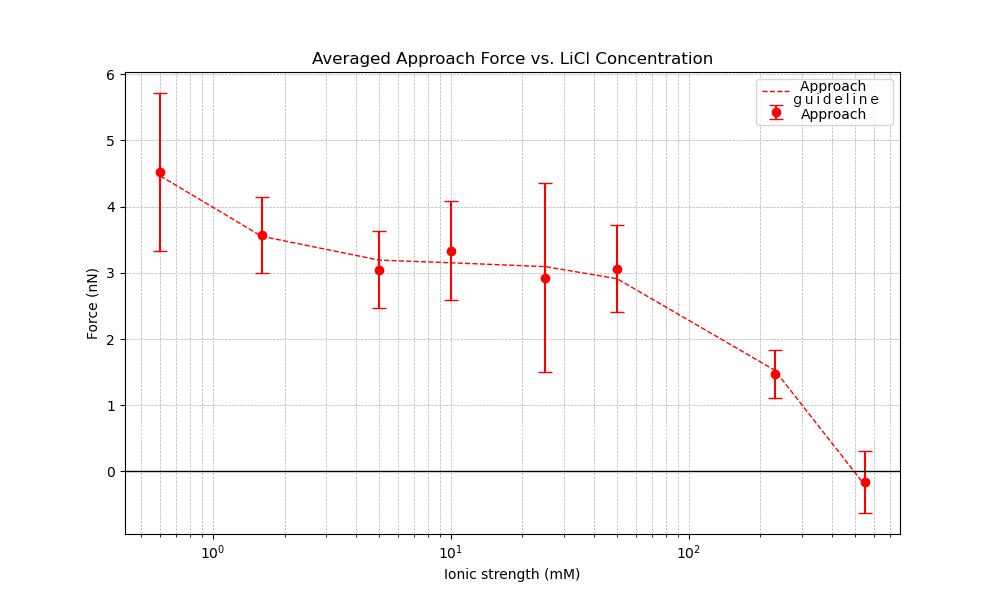
\includegraphics[width=1\linewidth]{chapter5/Average Approach.png}
    \caption{All sites' calculated force at contact with standard deviation error bars. There is an observed trend of increasing LiCl concentration leading to a decrease in repulsive force, until the repulsive force becomes attractive.}
    \label{fig:site1cont}
\end{figure}


The overall graph demonstrate the force at contact appears to decrease with increasing LiCl concentration. The reality for each of the sites is that they were exposed to different tips and different sites. As the AFM used was unable to save site locations, site 1, 2 and 3 aren't the same spacial location on the glass between salt concentrations.

An interesting observation however is in the error bars and thus the variability or uncertainty of the measurements. Larger error bars at middling concentrations, especially noticeable at 25mM, might suggest greater variability in the interaction forces measured at these points.

The dotted line was added to demonstrate the trend of the plots, which indicates that as salt concentration increases, the force requires for silica particles to come into contact decreases, eventually giving way to an attraction between the particles. This is likely due to the higher salt concentrations screening the electrostatic interactions. However, another interesting aspect is an observed plataeu between 5 - 50mM ionic strengths, potentially indicating a critical ion concentration needed to disrupt the electrostatic repulsion enough in this region.

These calculated forces are then expanded upon in chapter 7, with further analysis into potential reasons as to why these trends are observed.